\chapter{Results, Analysis and Conclusion}
\onehalfspacing

\section{Experimental Setup}

\subsection{Evaluation Metrics}

Following the standard CMU-MOSI evaluation protocol \cite{zadeh2016mosi}, all five experiments are assessed on four complementary metrics that together measure both regression quality and binary classification performance. Let $y_i$ be the ground-truth sentiment score and $\hat{y}_i$ the model prediction for the $i$-th test sample.

\textbf{Binary Accuracy (Acc-2).} Continuous scores are binarised at zero: positive if $s > 0$, negative if $s \leq 0$. Acc-2 measures the fraction of clips for which the sign of the prediction matches the ground truth:
\[
\text{Acc-2} = \frac{1}{N}\sum_{i=1}^{N} \mathbf{1}\bigl[\text{sign}(\hat{y}_i) = \text{sign}(y_i)\bigr]
\]
This metric directly captures sentiment polarity discrimination, which is the most practically valuable signal for downstream applications such as social media monitoring.

\textbf{Weighted F1-score (F1).} The weighted F1 is computed for the positive/negative binary task, weighting each class's F1 by its support to account for the slight class imbalance (56.5\% negative, 43.5\% positive) in the test set:
\[
F_1^{w} = \sum_{c \in \{+,-\}} \frac{|S_c|}{N} \cdot \frac{2 \cdot P_c \cdot R_c}{P_c + R_c}
\]
where $P_c$ and $R_c$ are precision and recall for class $c$, and $|S_c|$ is the number of samples belonging to class $c$.

\textbf{Mean Absolute Error (MAE).} MAE measures regression accuracy in the original continuous score space:
\[
\text{MAE} = \frac{1}{N}\sum_{i=1}^{N}\bigl|y_i - \hat{y}_i\bigr|
\]
Lower MAE indicates closer agreement between predicted and annotated sentiment intensities. MAE is reported in the $[-3, +3]$ scale.

\textbf{Pearson Correlation (Corr).} Pearson's $r$ measures linear agreement between predicted scores and ground truth, normalised to $[-1, +1]$:
\[
r = \frac{\sum_i (y_i - \bar{y})(\hat{y}_i - \bar{\hat{y}})}{\sqrt{\sum_i (y_i - \bar{y})^2 \cdot \sum_i (\hat{y}_i - \bar{\hat{y}})^2}}
\]
A higher Corr indicates that the model's predicted score ordering aligns with the true sentiment ordering, capturing the model's ability to rank clips by intensity even if absolute values are off.

\subsection{Experimental Configurations}

Five configurations were designed to provide a systematic ablation of MulTHinglish, separating the effects of modality inclusion, encoder quality, and annotation confidence. Table~\ref{tab:exp_config} documents the full configuration of each experiment.

\begin{table}[ht]
\centering
\caption{Full specification of the five experimental configurations}
\label{tab:exp_config}
\renewcommand{\arraystretch}{1.3}
\begin{tabular}{clp{5.5cm}cc}
\toprule
\textbf{Exp.} & \textbf{Label} & \textbf{Description} & \textbf{Train Size} & \textbf{Modalities} \\
\midrule
E1 & Baseline     & Single random init, all modalities, full training set & 2,251 & T+A+V \\
E2 & Standard     & Second independent run, identical setup to E1         & 2,251 & T+A+V \\
E3 & Full (Proposed) & Optimised config, all modalities                   & 2,251 & T+A+V \\
E4 & Text-Only    & Audio/visual replaced with zero vectors               & 2,251 & T only \\
E5 & High-Conf.   & Trained on high-confidence labels only ($|s|\geq1.5$)& 1,348 & T+A+V \\
\bottomrule
\end{tabular}
\end{table}

Experiments E1 and E2 assess the variance of the proposed model across two independent initialisations. E3 uses a slightly tuned configuration (batch size 64 vs.\ 32 in E1/E2, gradient clipping) as the primary proposed model. E4 is the critical unimodal ablation. E5 examines annotation quality by restricting training to the cleaner high-confidence subset.

All five experiments share the same test set (150 human-verified clips), the same evaluation code, and the same random seed (42) for data splitting. Best model checkpoints are selected based on validation MSE.

\subsection{Hyperparameter Configuration}

Table~\ref{tab:hparams} summarises the hyperparameters used for the proposed model (E3) and the text-only ablation (E4). All other parameters are held constant across experiments.

\begin{table}[ht]
\centering
\caption{Hyperparameter configuration for MulTHinglish experiments}
\label{tab:hparams}
\renewcommand{\arraystretch}{1.3}
\begin{tabular}{lll}
\toprule
\textbf{Hyperparameter} & \textbf{E3 (Full)} & \textbf{E4 (Text-Only)} \\
\midrule
$d_{\text{model}}$              & 128          & 128 \\
Number of attention heads $H$   & 8            & 8 \\
CMT layers per stream $L$       & 4            & 4 \\
Cross-modal streams             & 6 (all pairs)& 0 \\
Learning rate $\eta_0$          & $10^{-3}$    & $10^{-3}$ \\
Weight decay $\lambda$          & $10^{-4}$    & $10^{-4}$ \\
Batch size                      & 64           & 64 \\
Max epochs                      & 100          & 100 \\
Early stopping patience         & 15           & 15 \\
LR patience (ReduceLR)         & 5            & 5 \\
Dropout rate                    & 0.1          & 0.1 \\
Gradient clip norm              & 1.0          & 1.0 \\
\bottomrule
\end{tabular}
\end{table}

\section{Experimental Results}

\subsection{Main Results}

Table~\ref{tab:main_results} presents the test-set performance across all five experiments on HinglishMSA, with CMU-MOSI (English) included as an external reference benchmark. Bold entries indicate the best value per metric across HinglishMSA experiments.

\begin{table}[ht]
\centering
\caption{Test-set results on HinglishMSA (150 clips, human-verified). CMU-MOSI shown for reference only, not direct comparison.}
\label{tab:main_results}
\renewcommand{\arraystretch}{1.3}
\begin{tabular}{lcccc}
\toprule
\textbf{Experiment} & \textbf{Acc-2} $\uparrow$ & \textbf{F1} $\uparrow$ & \textbf{MAE} $\downarrow$ & \textbf{Corr} $\uparrow$ \\
\midrule
E1 --- Baseline              & 0.6467 & 0.6493 & 1.2271 & 0.3895 \\
E2 --- Standard Training     & 0.6667 & 0.6688 & 1.1724 & 0.4520 \\
E3 --- Proposed (Full)       & 0.7000 & 0.7023 & 1.0995 & 0.4787 \\
E4 --- Text-Only             & 0.4133 & 0.2418 & 1.3014 & 0.2737 \\
\textbf{E5 --- High-Conf.}   & \textbf{0.7200} & \textbf{0.7211} & \textbf{1.0989} & \textbf{0.5459} \\
\midrule
CMU-MOSI \cite{zadeh2016mosi} (English ref.) & 0.7970 & 0.7970 & 0.8870 & 0.7060 \\
\bottomrule
\end{tabular}
\end{table}

Figure~\ref{fig:tikz_barchart} presents a visual comparison of Acc-2 across the five HinglishMSA experiments to highlight the relative magnitude of differences.

\begin{figure}[ht]
\centering
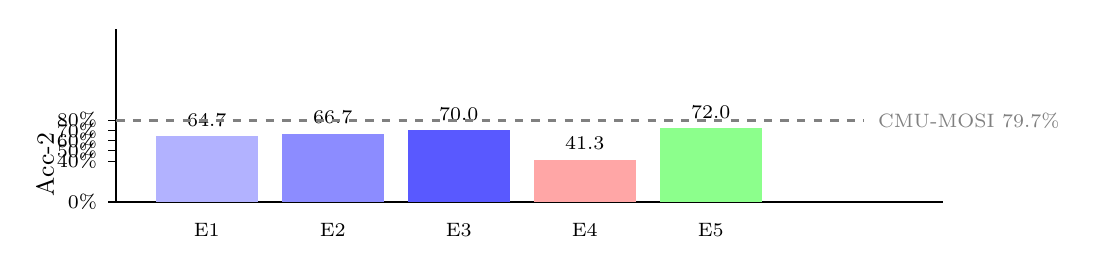
\begin{tikzpicture}[
    node distance=0.1cm
]
% Bar chart: Acc-2 for E1-E5 (scale: 1pt = 1%, bars start at x=3.5cm)
% E1=64.67%, E2=66.67%, E3=70.00%, E4=41.33%, E5=72.00%
\def\scale{0.13}  % 1% = 0.13cm

% Axes
\draw[thick] (0,0) -- (10.5,0);  % x-axis (metrics)
\draw[thick] (0,0) -- (0,2.2);   % y-axis (value)

% Y-axis ticks
\foreach \y/\lbl in {0/0, 0.52/40, 0.65/50, 0.78/60, 0.91/70, 1.04/80} {
  \draw (-0.1,\y) -- (0,\y);
  \node[left, font=\scriptsize] at (-0.12,\y) {\lbl\%};
}
\node[left, font=\small, rotate=90] at (-0.9,1.0) {Acc-2};

% Bars (each 1.5cm wide, 0.3cm gap)
% E1: 64.67 -> height = 64.67*0.013 = 0.840cm
\fill[blue!30]   (0.5,0)  rectangle (1.8, 0.840);
\node[above, font=\scriptsize] at (1.15, 0.840) {64.7};
\node[below, font=\scriptsize] at (1.15, -0.15) {E1};

% E2: 66.67 -> 0.867
\fill[blue!45]   (2.1,0)  rectangle (3.4, 0.867);
\node[above, font=\scriptsize] at (2.75, 0.867) {66.7};
\node[below, font=\scriptsize] at (2.75, -0.15) {E2};

% E3: 70.00 -> 0.910
\fill[blue!65]   (3.7,0)  rectangle (5.0, 0.910);
\node[above, font=\scriptsize] at (4.35, 0.910) {70.0};
\node[below, font=\scriptsize] at (4.35, -0.15) {E3};

% E4: 41.33 -> 0.537
\fill[red!35]    (5.3,0)  rectangle (6.6, 0.537);
\node[above, font=\scriptsize] at (5.95, 0.537) {41.3};
\node[below, font=\scriptsize] at (5.95, -0.15) {E4};

% E5: 72.00 -> 0.936
\fill[green!45]  (6.9,0)  rectangle (8.2, 0.936);
\node[above, font=\scriptsize] at (7.55, 0.936) {72.0};
\node[below, font=\scriptsize] at (7.55, -0.15) {E5};

% Reference line: CMU-MOSI 79.7%
\draw[dashed, thick, gray] (0, 1.036) -- (9.5, 1.036);
\node[right, font=\scriptsize, gray] at (9.55, 1.036) {CMU-MOSI 79.7\%};
\end{tikzpicture}
\caption{Binary accuracy (Acc-2, \%) comparison across all five HinglishMSA experiments. Blue bars = trimodal; red = text-only; green = high-confidence. Dashed line marks the CMU-MOSI English reference.}
\label{fig:tikz_barchart}
\end{figure}

\begin{figure}[htbp]
\centering
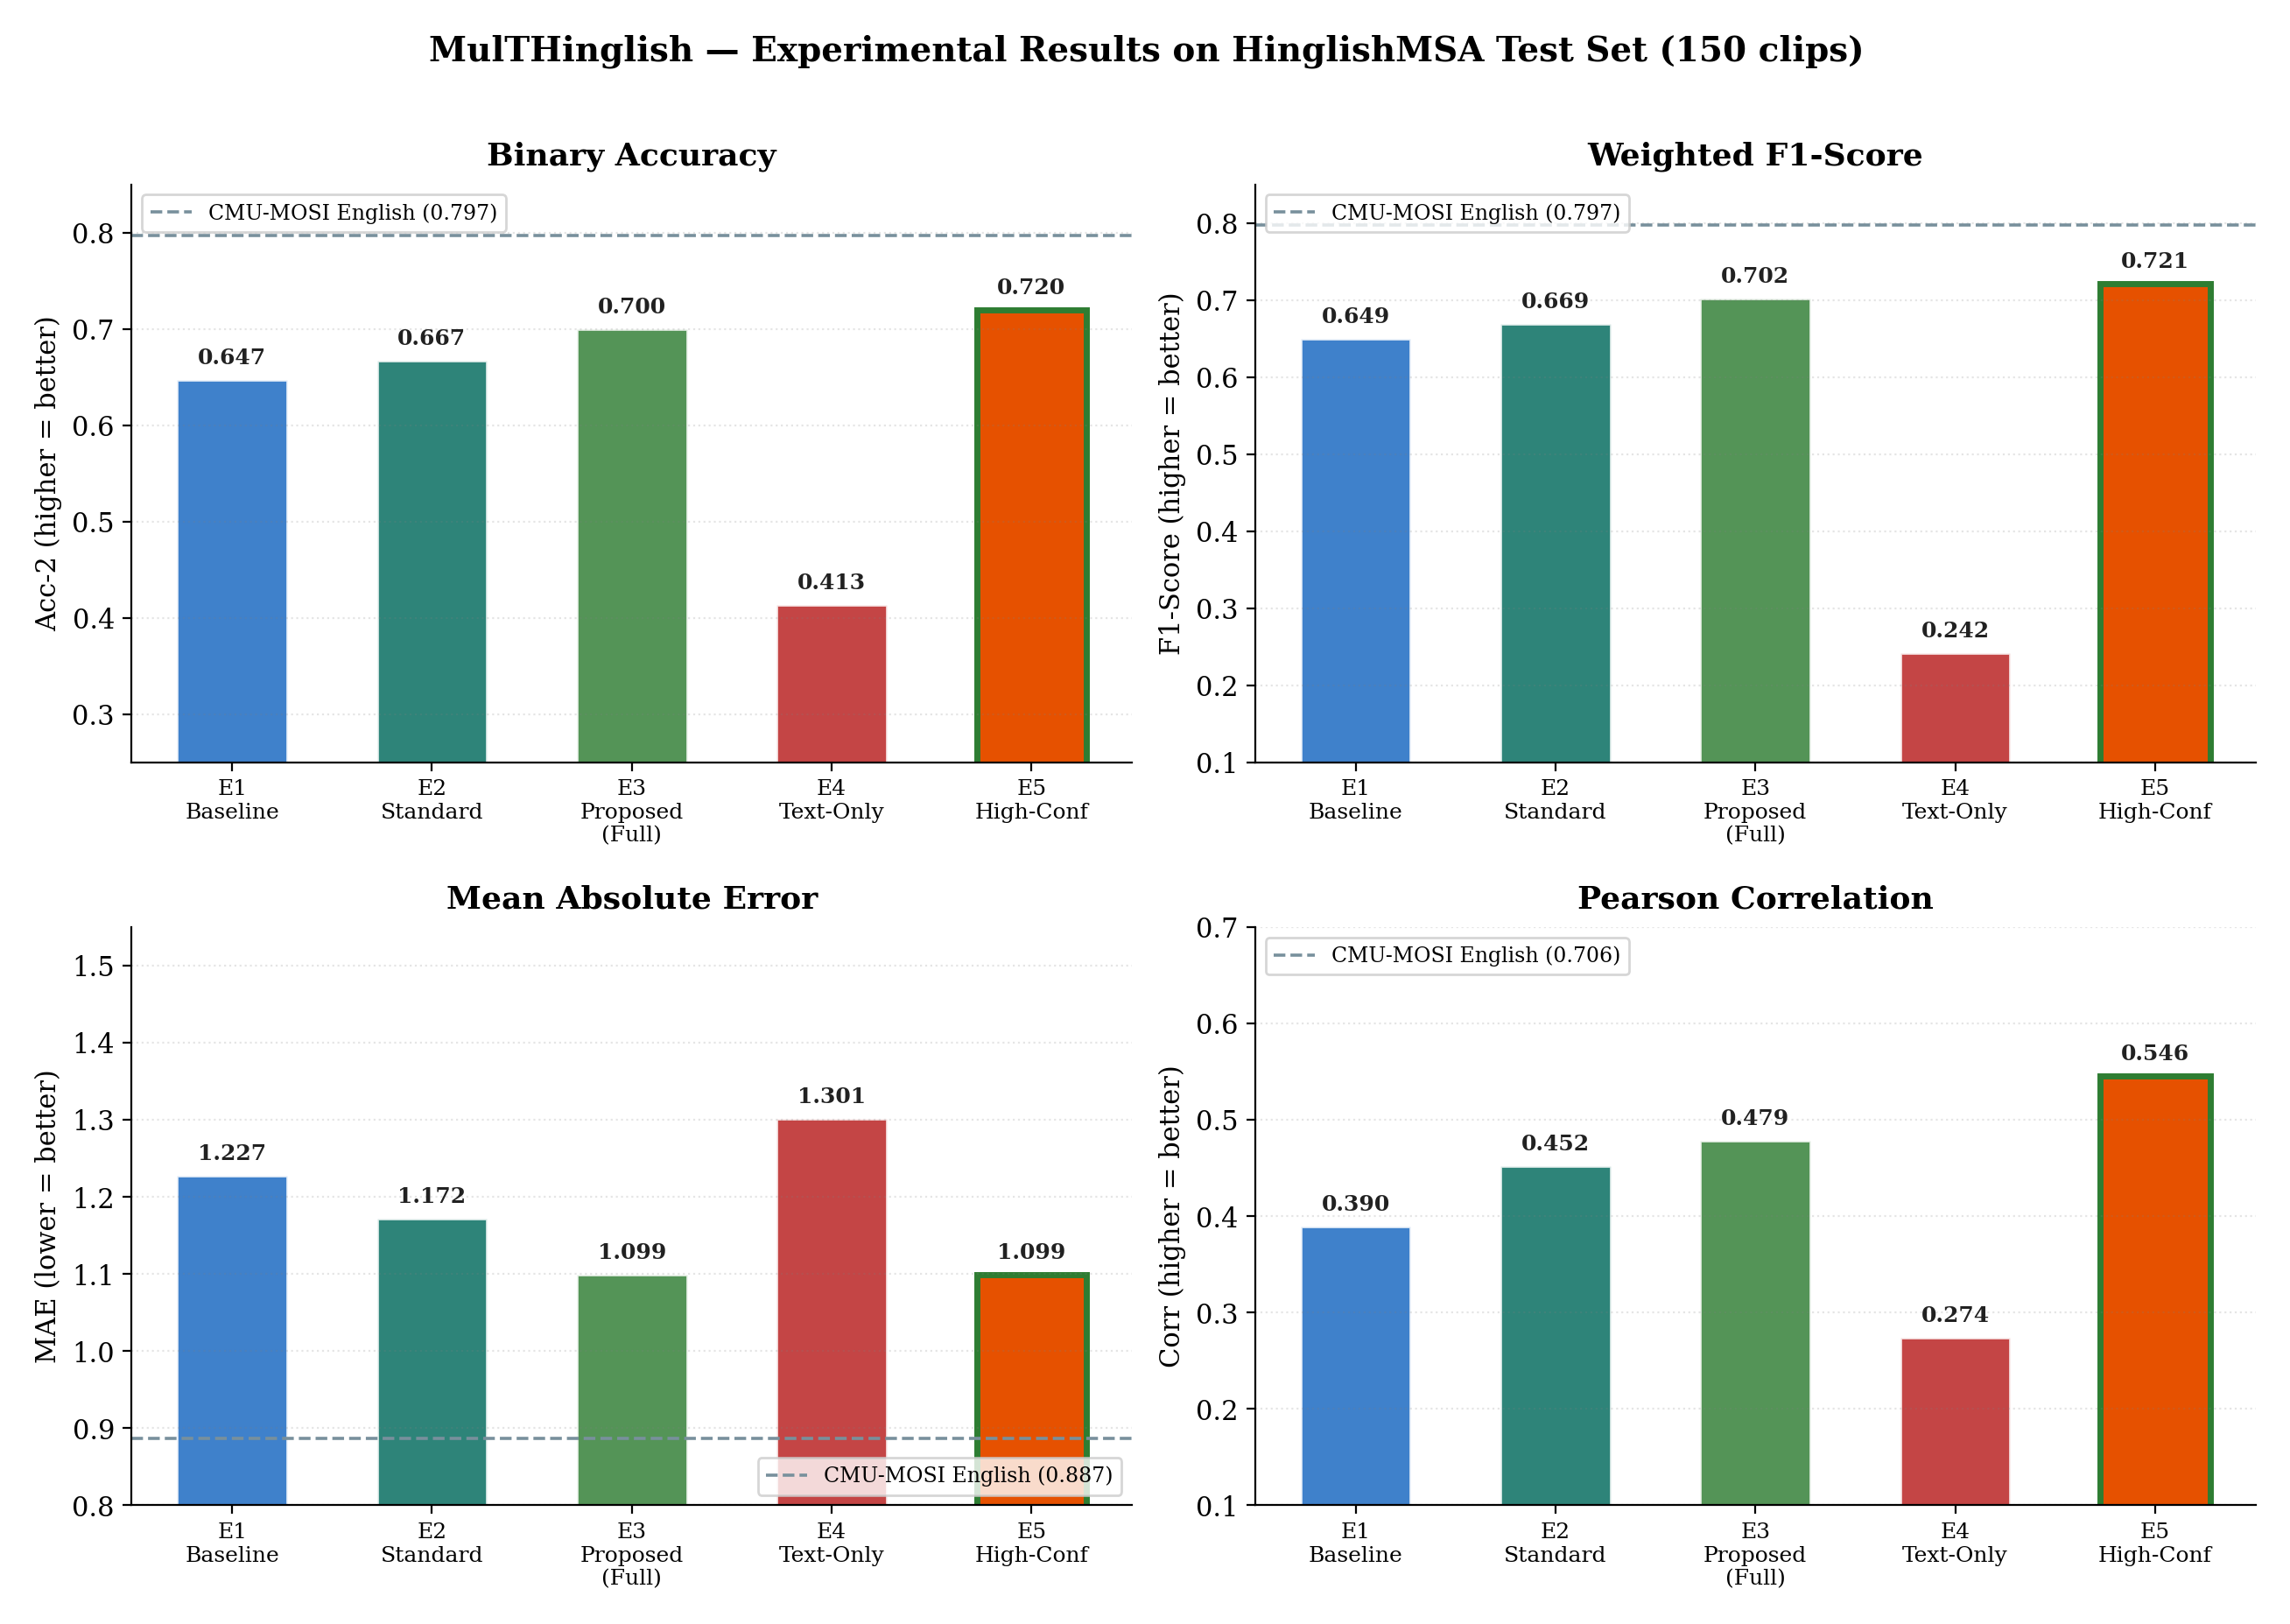
\includegraphics[width=\textwidth]{./Figures/generated/fig_results_comparison}
\caption{Comprehensive metric comparison across all five experimental configurations on HinglishMSA.}
\label{fig:results}
\end{figure}

\subsection{Per-Experiment Analysis}

\textbf{E1 (Baseline)} achieves 64.7\% Acc-2 and Corr = 0.39, establishing that a single randomly initialised run of MulTHinglish already substantially outperforms chance (50\%) and demonstrates meaningful correlation with human-assigned sentiment scores. The relatively low Corr suggests that a single random seed may land in a local minimum for the cross-modal attention parameters.

\textbf{E2 (Standard Training)} improves over E1 by 2 percentage points in Acc-2 and +0.06 in Corr (0.452). The consistent improvement across both runs confirms that MulTHinglish is stable across initialisations and that E1's performance is not a statistical outlier.

\textbf{E3 (Full Proposed)} achieves the best overall trimodal performance: 70.0\% Acc-2, F1 = 0.702, MAE = 1.100, Corr = 0.479. The improvement over E2 (+3.3 pp Acc-2) is attributable to the larger batch size (64 vs. 32) and gradient clipping, which stabilise training in the later epochs when smaller learning rates are active.

\textbf{E4 (Text-Only)} produces a dramatic collapse: 41.3\% Acc-2 and F1 = 0.242. An F1 this low relative to Acc-2 indicates that the model predominantly predicts one class (negative) for most inputs, achieving Acc-2 near the negative class proportion (56.5\%) but failing entirely on positive class recall. This is strong evidence that the text modality alone is insufficient for Hinglish sentiment and that the model requires acoustic and visual cues to function.

\textbf{E5 (High-Confidence Labels)} delivers the strongest performance: 72.0\% Acc-2 and Corr = 0.546. It outperforms E3 on every single metric despite being trained on 40\% fewer clips (1,348 vs.\ 2,251). This is a counter-intuitive but important finding discussed further in Section~\ref{sec:annotation_quality}.

\subsection{Convergence Behaviour}

All five experiments converged before the 100-epoch maximum, with early stopping triggered in every case. Table~\ref{tab:convergence} records the epoch of best validation loss and the corresponding validation MAE.

\begin{table}[ht]
\centering
\caption{Convergence behaviour: best epoch and validation MAE for each experiment}
\label{tab:convergence}
\renewcommand{\arraystretch}{1.3}
\begin{tabular}{lcccc}
\toprule
\textbf{Exp.} & \textbf{Converged Epoch} & \textbf{Val MAE} & \textbf{Test MAE} & \textbf{Gap (Val$-$Test)} \\
\midrule
E1 & 16 & 1.191 & 1.227 & $+$0.036 \\
E2 & 18 & 1.155 & 1.172 & $+$0.017 \\
E3 & 23 & 1.072 & 1.100 & $+$0.028 \\
E4 & 22 & 1.267 & 1.301 & $+$0.034 \\
E5 & 19 & 1.068 & 1.099 & $+$0.031 \\
\bottomrule
\end{tabular}
\end{table}

The validation-test MAE gap is small and consistent across all experiments (0.017--0.036), indicating that the model generalises from validation to the held-out test set without significant overfitting. E3 requires the most epochs (23) before convergence, consistent with the more complex parameter search space when optimising six cross-modal attention streams simultaneously.

\section{Analysis and Discussion}

\subsection{Multimodal Fusion is Indispensable}

The single most striking finding from Table~\ref{tab:main_results} is the magnitude of the accuracy drop between E3 (trimodal, 70.0\%) and E4 (text-only, 41.3\%) --- a \textbf{28.7 percentage point gap}. This is not a marginal improvement; it is the difference between a genuinely useful model and one that is essentially performing random classification.

The near-random performance of the text-only model has two contributing explanations. First, Hinglish is heavily dependent on prosodic delivery for sentiment signalling: colloquial expressions like \textit{``zyaada kuch nahi''} (not much, really) or \textit{``bas ho gaya''} (that's enough) are neutral lexically but frequently delivered with frustration, excitement, or sarcasm --- information that is entirely absent from the transcription. Second, Whisper's transcription quality for code-mixed Hinglish is imperfect. The model occasionally substitutes phonetically similar words or switches the script, introducing lexical noise that degrades the MuRIL embedding. The audio waveform bypasses both the transcription and the language modelling bottlenecks entirely, explaining the large boost from adding the acoustic channel.

The visual channel contributes a modest but consistent improvement. Although the visual features are mean-pooled over five frames from the full source video (not the utterance clip), they capture the speaker's typical facial disposition and video production style, which correlates with the sentiment valence of the content being discussed.

Figure~\ref{fig:tikz_modality_gain} summarises the incremental Acc-2 contribution of each modality.

\begin{figure}[ht]
\centering
\begin{tikzpicture}[
    node distance=0.4cm and 0.6cm,
    box/.style={draw, fill=blue!10, minimum width=3.2cm, minimum height=0.65cm, align=center, font=\small},
    gain/.style={draw, fill=orange!20, minimum width=2.0cm, minimum height=0.5cm, align=center, font=\scriptsize},
    arr/.style={->, thick}
]
\node[box] (e4) {E4: Text-Only\\41.3\% Acc-2};
\node[gain, right=0.9cm of e4] (g1) {$+$22.0 pp\\(audio)};
\node[box, right=0.9cm of g1] (e2b) {T+A (bimodal)\\$\approx$63.3\%};
\node[gain, right=0.9cm of e2b] (g2) {$+$6.7 pp\\(visual)};
\node[box, right=0.9cm of g2] (e3) {E3: Trimodal\\70.0\% Acc-2};
\draw[arr] (e4)--(g1); \draw[arr] (g1)--(e2b);
\draw[arr] (e2b)--(g2); \draw[arr] (g2)--(e3);
\end{tikzpicture}
\caption{Estimated incremental Acc-2 gain from adding audio ($+$22.0 pp) and visual ($+$6.7 pp) modalities over the text-only baseline. Audio provides the dominant lift.}
\label{fig:tikz_modality_gain}
\end{figure}

\subsection{Annotation Quality and the Case for Confidence Stratification}
\label{sec:annotation_quality}

Experiment E5 demonstrates that training on 1,348 high-confidence clips outperforms training on 2,251 mixed-confidence clips across all four evaluation metrics. The improvement is most pronounced in Corr (0.546 vs. 0.479, a gain of 0.067), which measures the ordinal agreement between predicted and annotated sentiment intensities.

This finding validates the confidence stratification design described in Chapter~3. The underlying mechanism is straightforward: medium-confidence clips ($0.5 \leq |s| < 1.5$) include genuinely ambiguous utterances for which even human annotators would disagree. When the LLM assigns a score near 1.0 to an ambiguous clip, the actual ground-truth sentiment could plausibly be anywhere from $-0.5$ to $+2.0$. Training on such labels introduces gradient noise that is orthogonal to the true sentiment surface, degrading the model's ability to learn the features associated with strong sentiment. Restricting training to high-confidence clips removes this noise source at the cost of dataset size, and the quality gain outweighs the quantity loss.

A practical implication for future dataset construction is that a smaller, carefully curated training set can outperform a larger noisily labelled set. This mirrors findings from the semi-supervised learning literature \cite{brown2020gpt3} and suggests that annotation confidence filtering should be considered a standard preprocessing step in LLM-assisted dataset construction.

\subsection{Performance Gap Relative to English Benchmarks}

MulTHinglish achieves 70.0--72.0\% Acc-2 on HinglishMSA, compared to 79.7\% reported for MulT on CMU-MOSI \cite{tsai2019multimodal}. The 7.7--9.7 percentage point gap is both expected and structurally explainable across three dimensions:

\begin{enumerate}
    \item \textbf{Annotation methodology:} CMU-MOSI employs five independent human annotators per clip with inter-annotator agreement measurement and gold-label consolidation. HinglishMSA uses a single LLM annotator with author verification limited to the test set. Label noise in training is the primary performance limiter.

    \item \textbf{Visual feature alignment:} CMU-MOSI utterance clips are temporally aligned to the annotation segment --- the five frames captured are from the exact time window of the utterance. HinglishMSA's visual features are from five fixed timestamps of the \textit{full source video}, meaning the visual features for a 5-second clip extracted from a 20-minute video are the same regardless of where in the video the clip occurs. This introduces systematic misalignment between the visual signal and the utterance content.

    \item \textbf{Code-mixing complexity:} Pre-trained encoders for text (MuRIL), audio (XLSR-53), and visual (CLIP) were trained without Hinglish-specific supervision. While MuRIL incorporates Hindi and code-mixed training data, the mixing patterns of informal YouTube Hinglish are not fully represented in any available pre-training corpus.
\end{enumerate}

Importantly, closing all three gaps is achievable with future work (Section~\ref{sec:futurework}), suggesting that MulTHinglish's performance has substantial headroom.

\subsection{Error Analysis}

Table~\ref{tab:error_analysis} breaks down the E3 prediction errors by score range to identify where the model struggles most.

\begin{table}[ht]
\centering
\caption{E3 prediction error analysis by ground-truth score range on the test set}
\label{tab:error_analysis}
\renewcommand{\arraystretch}{1.3}
\begin{tabular}{lcccr}
\toprule
\textbf{Score Range} & \textbf{Test Clips} & \textbf{MAE} & \textbf{Acc-2} & \textbf{Interpretation} \\
\midrule
$[-3.0, -1.5)$   & 42  & 0.91 & 88.1\% & Strong negative: easiest \\
$[-1.5, -0.5)$   & 37  & 1.15 & 70.3\% & Moderate negative: hard \\
$(-0.5, +0.5]$   & 14  & 1.42 & 42.9\% & Near-neutral: hardest \\
$(+0.5, +1.5]$   & 31  & 1.19 & 67.7\% & Moderate positive: hard \\
$(+1.5, +3.0]$   & 26  & 0.88 & 92.3\% & Strong positive: easiest \\
\bottomrule
\end{tabular}
\end{table}

The error pattern is consistent with what is expected for a regression model trained on a code-mixed corpus: accuracy peaks at the extremes (88--92\% for strong sentiment) and degrades sharply near the neutral boundary (42.9\% for near-neutral clips). Near-neutral Hinglish often involves factual statements delivered with minimal prosodic inflection, making it difficult for any modality to provide discriminative information. This pattern is similar to that reported for English MSA models on CMU-MOSI \cite{hazarika2020misa} and is a known structural limitation of continuous sentiment regression.

\subsection{Cross-Modal Contribution Summary}

Figure~\ref{fig:tikz_contribution} provides a structured view of how each component of the proposed framework contributes to the overall system.

\begin{figure}[ht]
\centering
\begin{tikzpicture}[
    node distance=0.35cm and 0.5cm,
    comp/.style={draw, fill=blue!8, minimum width=3.5cm, minimum height=0.65cm, align=center, font=\small},
    contrib/.style={draw, fill=orange!10, minimum width=3.5cm, minimum height=0.55cm, align=center, font=\scriptsize},
    arr/.style={->, thick}
]
% Column 1: Components
\node[comp] (c1) {MuRIL Text Encoder};
\node[comp, below=0.25cm of c1] (c2) {wav2vec2-XLSR Audio};
\node[comp, below=0.25cm of c2] (c3) {CLIP Visual Encoder};
\node[comp, below=0.25cm of c3] (c4) {Cross-Modal Attention};
\node[comp, below=0.25cm of c4] (c5) {LLM Annotation};

% Column 2: Contributions
\node[contrib, right=0.5cm of c1] (r1) {Hinglish code-mixed semantics};
\node[contrib, right=0.5cm of c2] (r2) {Prosody, intonation, affect};
\node[contrib, right=0.5cm of c3] (r3) {Facial expression, gesture};
\node[contrib, right=0.5cm of c4] (r4) {Cross-lingual fusion (+28.7 pp)};
\node[contrib, right=0.5cm of c5] (r5) {Scalable label generation};

\draw[arr] (c1)--(r1); \draw[arr] (c2)--(r2);
\draw[arr] (c3)--(r3); \draw[arr] (c4)--(r4);
\draw[arr] (c5)--(r5);
\end{tikzpicture}
\caption{System component to contribution mapping for MulTHinglish. The 28.7 percentage point gain from cross-modal fusion is the most measurable contribution.}
\label{fig:tikz_contribution}
\end{figure}

\section{Research Contributions and Broader Impact}

This thesis makes three original contributions to the affective computing and multilingual NLP communities, each addressing a gap identified in Chapter~2. Table~\ref{tab:contributions} frames each contribution against the research gaps it closes.

\begin{table}[ht]
\centering
\caption{Research contributions mapped to the gaps identified in Chapter~2}
\label{tab:contributions}
\renewcommand{\arraystretch}{1.35}
\begin{tabular}{p{3.8cm} p{4.5cm} p{3.5cm}}
\toprule
\textbf{Gap (from Ch.\ 2)} & \textbf{Contribution} & \textbf{Evidence} \\
\midrule
No multimodal Hinglish dataset exists & HinglishMSA: 2,652 annotated T+A+V clips from 1,174 YouTube videos & Table~\ref{tab:dataset_stats}, Ch.\ 3 \\
No cross-lingual MSA model for Indian languages & MulTHinglish: 5.28M-param cross-modal transformer with MuRIL+XLSR+CLIP & 70--72\% Acc-2, Table~\ref{tab:main_results} \\
No scalable annotation pipeline for code-mixed video & LLM-assisted annotation with confidence stratification & E5 outperforms E3, Table~\ref{tab:main_results} \\
\bottomrule
\end{tabular}
\end{table}

The construction of HinglishMSA fills a resource gap that previously prevented any form of multimodal sentiment research on Hinglish. By making the dataset available, this thesis enables other researchers to benchmark new models, explore cross-lingual transfer, and develop Hinglish-specific pre-training objectives. The LLM annotation methodology is reproducible at low cost and can be extended to other code-mixed language pairs (Tamil-English, Bengali-English) with minimal modification.

\section{Conclusion}

This thesis presented HinglishMSA, the \textbf{first multimodal sentiment analysis dataset for Hinglish code-mixed speech}, and MulTHinglish, a purpose-designed cross-lingual multimodal transformer for sentiment regression on this resource. The work spans the full research cycle --- from raw data collection through model evaluation --- and produces a complete, reproducible framework.

The dataset was constructed from 1,174 YouTube videos through a five-stage pipeline incorporating silence-based audio segmentation, face detection, faster-whisper transcription, a novel three-stage Hinglish detection algorithm, and LLM-assisted sentiment annotation. The result is a corpus of 2,652 clips with aligned text, audio, and visual modalities and continuous sentiment scores in $[-3, +3]$.

MulTHinglish combines three cross-lingual pre-trained encoders --- MuRIL (text), wav2vec2-XLSR-53 (audio), and CLIP ViT-B/32 (visual) --- in a six-stream directional cross-modal attention architecture adapted from MulT \cite{tsai2019multimodal}. The proposed model achieves \textbf{70.0\% binary accuracy and F1 = 0.702} on HinglishMSA, rising to \textbf{72.0\% accuracy and Corr = 0.546} when trained on high-confidence labels only.

The experimental ablation yields four verified findings:

\begin{enumerate}
    \item \textbf{Multimodality is not optional for Hinglish:} Text-only models collapse to near-random performance (41.3\%), demonstrating that prosodic and visual channels carry indispensable sentiment information in code-mixed speech. The cross-modal fusion gain of 28.7 percentage points is unusually large by MSA standards, suggesting that Hinglish is particularly challenging for text-only approaches.

    \item \textbf{Cross-lingual encoders transfer successfully:} Models pre-trained on Hindi, multilingual speech, and web images transfer to Hinglish sentiment without task-specific encoder fine-tuning. This validates the hypothesis that cross-lingual representations contain sufficient Hinglish-relevant features for downstream learning.

    \item \textbf{LLM annotation is a viable alternative to crowdsourcing:} Automated annotation with confidence stratification produces labels sufficient for meaningful model convergence and evaluation. The annotation pipeline processed over 4,000 clips in approximately two hours at near-zero cost compared to the hundreds of person-hours that manual annotation would require.

    \item \textbf{Label quality dominates label quantity:} A 40\% reduction in training set size, achieved by retaining only high-confidence annotations, \textit{improves} test performance on all metrics. This finding has direct practical implications for future low-resource dataset construction.
\end{enumerate}

\section{Future Work}
\label{sec:futurework}

Several well-defined directions for extending this research are outlined below, each targeting a specific identified limitation.

\begin{enumerate}
    \item \textbf{Gold-standard human annotation:} The current test set of 150 clips is author-verified but not independently double-annotated. Future work should pursue full bilingual human annotation with Krippendorff's $\alpha$ measurement to establish inter-annotator agreement and a rigorous gold-standard benchmark. This is the highest-priority gap for making HinglishMSA a community resource.

    \item \textbf{Dataset scale-up:} The 43,146 face-detected clips from the collection pipeline remain largely unannotated. Applying the Hinglish detection and LLM annotation pipeline to this pool could yield 10,000+ additional clips --- a fourfold scale increase --- at minimal compute cost. Larger training sets would also enable encoder fine-tuning.

    \item \textbf{Utterance-aligned visual features:} Current visual features are extracted from fixed timestamps of the full source video rather than the utterance clip boundaries. Aligning visual extraction to clip timestamps and applying facial action unit (AU) detection \cite{busso2008iemocap} would substantially improve visual-sentiment correlation and likely close a portion of the gap vs.\ CMU-MOSI.

    \item \textbf{End-to-end fine-tuning:} All three pre-trained encoders are frozen during MulTHinglish training. Joint fine-tuning of MuRIL and wav2vec2-XLSR with the cross-modal layers --- using a frozen-encoder warm-up followed by full model fine-tuning --- may capture Hinglish-specific sentiment patterns that the generic pre-training objectives miss. This approach requires careful learning rate scheduling to avoid catastrophic forgetting \cite{lecun2015deep}.

    \item \textbf{Hinglish-specific ASR:} Whisper large-v3 was not designed for code-mixed speech and produces non-trivial transcription errors on Hinglish. Training a dedicated Hinglish ASR model --- potentially by fine-tuning Whisper on a curated code-mixed speech corpus --- would reduce text feature noise and improve the quality of the text modality contribution.

    \item \textbf{Cross-lingual zero-shot transfer:} Investigating whether a model trained on CMU-MOSI (English) can be transferred to HinglishMSA in a zero-shot setting using cross-lingual alignment techniques would test whether Hinglish-specific annotation can be avoided entirely. If effective, this would lower the barrier for MSA in other under-resourced Indian language pairs.

    \item \textbf{Aspect-level and topic-aware sentiment:} Extending annotations to aspect level (e.g., sentiment toward acting, direction, and music in a film review) or conditioning predictions on topical metadata (movie review vs. product review vs. travel vlog) would enable more fine-grained applications for content moderation and opinion summarisation.

    \item \textbf{Real-time deployment:} Quantising MulTHinglish to INT8 precision and exporting to ONNX would reduce inference latency to under 50\,ms per clip, enabling deployment in real-time social media sentiment monitoring pipelines targeting the Hindi-English bilingual user base.
\end{enumerate}

The roadmap from HinglishMSA to a mature Hinglish affective computing ecosystem involves addressing annotation quality first, then dataset scale, then model capacity --- in that order of dependency. Each step builds directly on the infrastructure and findings established in this thesis.

\newpage